\begin{abcliste}
\abc Auf den Bob wirken die Gewichtskraft und die Normalkraft der Eisbahn; die Reibung auf dem Eis ist klein. In der Kurve ist die Bahn stark überhöht: Die Normalkraft steht senkrecht auf der geneigten Bahnwand und hat eine waagrechte Komponente zum Kurvenmittelpunkt. Die Resultierende aus Normalkraft und Gewichtskraft ist die Zentripetalkraft.

\begin{center}
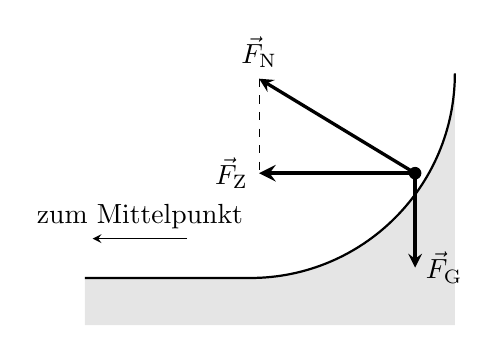
\begin{tikzpicture}[>=stealth]
 \fill[gray!20] (-1.5,-1.0) -- (0.6,-1.0) arc (-90:0:2.6) -- (3.2,-1.6) -- (-1.5,-1.6) -- cycle;
 \draw[thick] (-1.5,-1.0) -- (0.6,-1.0) arc (-90:0:2.6);
 \fill (2.695,0.331) circle (0.08);
 \draw[->, very thick] (2.695,0.331) -- (0.714,1.531) node[above] {$\vec F_\mathrm{N}$};
 \draw[->, very thick] (2.695,0.331) -- (2.695,-0.869) node[right] {$\vec F_\mathrm{G}$};
 \draw[dashed] (0.714,1.531) -- (0.714,0.331);
 \draw[->, ultra thick] (2.695,0.331) -- (0.714,0.331) node[left] {$\vec F_\mathrm{Z}$};
 \draw[->] (-0.2,-0.5) -- (-1.4,-0.5) node[midway, above] {zum Mittelpunkt};
\end{tikzpicture}
\end{center}

\abc Die nötige Zentripetalkraft ist
\begin{align}
 F_\mathrm{Z} &= \FBoF = \frac{\mBo\cdot\left(\vBo\right)^2}{\rBo} = \FBo \approx \result{\FBoP{3}{2}}
\end{align}
Das ist deutlich mehr als die Gewichtskraft des Bobs.
\end{abcliste}
